\documentclass[conference]{IEEEtran}
\IEEEoverridecommandlockouts

\usepackage{cite}
\usepackage{amsmath,amssymb,amsfonts}
\usepackage{algorithmic}
\usepackage{algorithm}
\usepackage{graphicx}
\usepackage{textcomp}
\usepackage{xcolor}
\usepackage{tikz}
\usepackage{threeparttable} % Supports footnotes inside tables
\usepackage{graphicx} % Add this to your preamble
\usepackage{tabularx} % Add this to your preamble
\usepackage{comment}
\usepackage{float}
\usepackage{diagbox}
\usepackage{hyperref}
\hypersetup{
    colorlinks=true,
    linkcolor=blue,
    citecolor=blue,
    urlcolor=blue
}
%\usepackage[skip=5pt]{caption} % Add this in the preamble
\setlength{\textfloatsep}{8pt} 

%\usetikzlibrary{shapes, arrows, positioning}

\bibliographystyle{IEEEtran}

\begin{document}

\title{Hardware-Efficient Three-Input Fuzzy MPPT for PV Battery Charger ICs}

\author{\IEEEauthorblockN{Mehmet Gök, Kemal Ozanoglu, and Günhan Dündar}
\IEEEauthorblockA{\small{Department of Electrical and Electronics Engineering, Bogazici University, Istanbul, Türkiye}}
}
\maketitle

\begin{abstract} Maximizing power extraction from photovoltaic (PV)
    arrays under dynamic environmental conditions is critical
    for battery charging. Conventional MPPT (Maximum Power Point
    Tracking) algorithms suffer
    from slow transients and steady-state oscillations.
    To address these limits, this paper presents an
    ASIC-oriented FLC (fuzzy logic controller) modeled in
    MATLAB/Simulink using three parameters:
    $\Delta V_{pv}$, $\Delta I_{out}$, and $V_{pv}$.
    To avoid complex hardware division in the FLC,
    a hardware-efficient method utilizing look-up
    tables and bitwise shift operations is proposed.
    Simulation results show a 
    steady-state PV tracking efficiency exceeding
    99\%, a buck converter efficiency of $\sim$95\%,
    and millisecond-level transient recovery during
    sudden irradiance drops, achieving near-optimal performance
    with significantly reduced complexity.
\end{abstract}

\begin{IEEEkeywords}
Fuzzy Logic Control (FLC), Maximum Power Point Tracking (MPPT),
Photovoltaic (PV) Systems, Multi-Input Fuzzy Inference,
Battery Charging, MPPT Optimization
\end{IEEEkeywords}

\section{Introduction}
\label{sec:intro}
The integration of photovoltaic (PV) systems
is critical for sustainable power generation,
but PV power output is non-linear and depends
heavily on dynamic environmental conditions.
MPPT algorithms are
essential to maximize energy extraction,
reduce energy waste, and improve battery charging
efficiency.

Although conventional algorithms such as Perturb
and Observe (P\&O) and Incremental Conductance (IC) are
widely used \cite{po_ic}, they are often enhanced with 
intelligent control techniques such as fuzzy logic
to handle rapidly changing conditions \cite{fuzzy_review}. 

In this work, we introduce a hardware-efficient,
three-input fuzzy MPPT architecture that combines a 
deterministic boundary safety override with multi
-input fuzzy logic tracking. By processing $\Delta V_{pv}$,
$\Delta I_{out}$, and $V_{pv}$ using only simple
look-up tables and bitwise shifts, the design eliminates
complex arithmetic blocks, making it ideal for
low-cost power management ICs.
The system overview is shown in Figure 
\ref{fig:matlab_overview}.

\begin{figure}[ht]
\centering

\includegraphics[width=\columnwidth]{./images/matlab/matlab_model_overview.png}
\caption{Simulink model overview of the proposed fuzzy logic-based MPPT system for PV battery charger.}
\label{fig:matlab_overview}
\end{figure}

The remainder of this paper is organized as follows:
Section \ref{sec:architecture} details the system architecture including the PV model and buck converter,
Section \ref{sec:fuzzy_controller} describes the proposed fuzzy logic controller,
Section \ref{sec:results} presents the simulation results,
and Section \ref{sec:conclusion} concludes.

\section{System Architecture}
\label{sec:architecture}

This project aims to charge a $\sim$12V car battery
using PV modules that have a Maximum Power Point (MPP)
voltage of $\sim$30V.
Because the PV voltage is significantly higher than
the target battery voltage, a buck converter
is chosen to efficiently step down the voltage.
MATLAB/Simulink is chosen as the simulation environment 
for implementing and validating the proposed system 
(Figure \ref{fig:matlab_overview}).

\subsection{Photovoltaic Panel Model}
\label{subsec:pv}

The PV model's example I-V \& Power characteristics,
based on De Soto et al. \cite{DeSoto2006}, are shown 
in Figure \ref{fig:pv_curves}. As observed in the 
figure, despite varying irradiance conditions, the 
MPP is compressed into a narrow voltage range 
(around 30V). 

\begin{figure}[ht]
\centering

\includegraphics[width=0.95\columnwidth]{./images/matlab/pv_IV&powercurves.jpg}
\caption{I-V and power characteristics of the photovoltaic panel under various irradiance conditions.}
\label{fig:pv_curves}
\end{figure}

Our tracking goal is to maintain 
system operation within this narrow target range. 
The controller adjusts the converter's 
duty cycle to modulate the PV panel impedance 
and maintain optimal operation. The inference 
mechanism details are provided in 
Section \ref{sec:fuzzy_controller}.

\subsection{Buck Converter}
\label{subsec:buck_converter}

\subsubsection{Buck Converter Specifications}
\label{subsec:buck_specs}

The buck converter specifications, derived from \cite{EricksonBook,RashidBook,TIReport} and optimized for efficient power conversion, are presented in Table \ref{tab:buck_converter_specs}. Parasitics of passive components are excluded in this system-level model.

\begin{table}[ht]
\centering
\caption{Buck Converter Specifications}
\label{tab:buck_converter_specs}
\begin{tabular}{|l|c|c|}
\hline
\textbf{Parameter} & \textbf{Symbol} & \textbf{Value} \\
\hline
Input Voltage (MPP) & $V_{in}$ & 30.6 V \\
\hline
Output Voltage (Battery) & $V_{out}$ & 14.4 V \\
\hline
Switching Frequency & $f_{sw}$ & 500 kHz \\
\hline
Sampling Frequency & $f_{sample}$ & 20 kHz \\
\hline
Inductance & $L$ & 2.6 $\mu$H \\
\hline
Input Capacitance & $C_{in}$ & 47 $\mu$F \\
\hline
Parasitic Resistance of Switch & $R_{sw}$ & 10 m$\Omega$ \\
\hline
Diode Forward Voltage & $V_f$ & 0.5 V \\
\hline
\end{tabular}
\end{table}

\section{Fuzzy Logic Controller}
\label{sec:fuzzy_controller}

The fuzzy logic controller takes three input parameters ($\Delta V_{pv}$, $\Delta I_{out}$, and $V_{pv}$) to compute the duty cycle change ($\Delta D$). 
The block diagram is shown in Figure \ref{fig:fuzzy_diagram}.

\begin{figure}[ht]
\centering
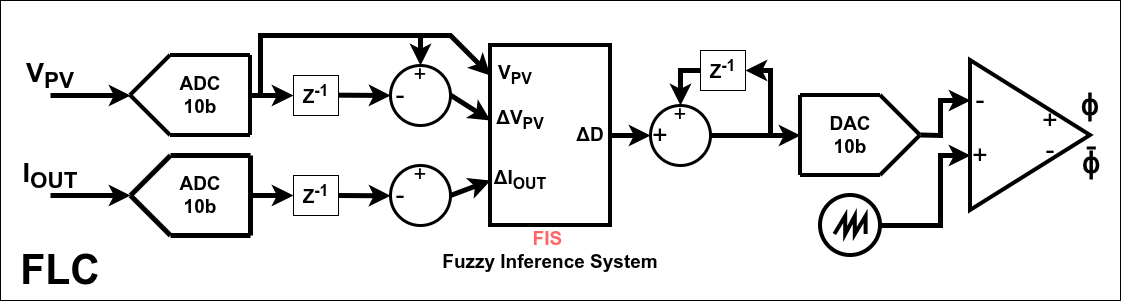
\includegraphics[width=\columnwidth]{./images/matlab/fuzzy_controller_block_diagram.png}
\caption{Fuzzy logic controller block diagram showing the three phases of operation.}
\label{fig:fuzzy_diagram}
\end{figure}

Input sampling and final duty adjustment are straightforward processes. Therefore, this section focuses on the key operations: inference, fuzzification, and defuzzification.

\subsection{Inference}
This phase evaluates IF-THEN rules using the \textbf{min} 
operator for logical AND. 
The inputs $\Delta V_{pv}$ and $\Delta I_{out}$ are 
mapped to three fuzzy sets: \textbf{Negative}, 
\textbf{Zero}, and \textbf{Positive}. $V_{pv}$ is 
mapped to \textbf{Low\_Voltage}, \textbf{Optimal\_Voltage}
, and \textbf{High\_Voltage}. The output $\Delta D$ 
is mapped to five sets: \textbf{Big\_Decrease}, 
\textbf{Decrease}, \textbf{Hold}, \textbf{Increase}, 
and \textbf{Big\_Increase}.

3 inputs with 3 fuzzy sets would yield a total of  
27 ($3 \times 3 \times 3$) rules. However, to reduce
silicon area, we streamline this to 11 rules. There is
another advantage to this approach: it prevents local minima
trapping by prioritizing the absolute voltage level 
($V_{pv}$) over the incremental changes ($\Delta V_{pv}$ 
and $\Delta I_{out}$).
When $V_{pv}$ is outside the MPP range, two boundary 
safety rules override and suppress the others 
(Table \ref{tab:fuzzy_rules_safety}). 
When $V_{pv}$ is optimal, only the 9 rules 
based on voltage and current variations are 
evaluated (Table \ref{tab:fuzzy_rules_optimal}). 
This approach maintains the advantage of avoiding 
local minima while optimizing the 
hardware implementation. Effectively FLC is constructed 
with P\&O enhancement.

\begin{table}[htbp]
    \centering
    \caption{Fuzzy Logic Safety Rules}
    \begin{tabular}{|c|c|}
        \hline
        \textbf{PV Voltage ($V_{pv}$)} & \textbf{Output ($\Delta D$)} \\
        \hline
        \textbf{Low\_Voltage} & \textbf{Big\_Decrease} \\
        \hline
        \textbf{High\_Voltage} & \textbf{Big\_Increase} \\
        \hline
    \end{tabular}
    \label{tab:fuzzy_rules_safety}
\end{table}

\begin{table}[htbp]
    \centering
    \caption{Fuzzy Logic Rules for Optimal Range}
    \begin{tabular}{|c|c|c|c|}
        \hline
        \diagbox{$dI$}{$dV$} & \textbf{Negative} & \textbf{Zero} & \textbf{Positive} \\
        \hline
        \textbf{Negative} & \textbf{Decrease} & \textbf{Hold} & \textbf{Increase} \\
        \hline
        \textbf{Zero} & \textbf{Hold} & \textbf{Hold} & \textbf{Hold} \\
        \hline
        \textbf{Positive} & \textbf{Increase} & \textbf{Hold} & \textbf{Decrease} \\
        \hline
    \end{tabular}
    \label{tab:fuzzy_rules_optimal}
\end{table}

\subsection{Fuzzification}
The hardware implementation utilizes three primary types of membership functions: Z-shaped, S-shaped, and Triangular-shaped. The degree of membership is found by mapping the crisp digital 10-bit input to a linear segment. The membership range value is chosen as 0 to 255 ($M=255$). It is extracted using linear interpolation. To avoid complex division, we round the denominator to the nearest power of 2, which allows us to replace the division with a simple right bitwise shift. The membership calculation procedure is summarized in Algorithm \ref{alg:mf_interpolation}.

\begin{algorithm}[H]
\caption{Hardware-Efficient Linear Interpolation for Membership Functions}
\label{alg:mf_interpolation}
\begin{algorithmic}[1]
\REQUIRE Crisp input $x$, Thresholds $A$ and $B$, Max Output $M$
\ENSURE Membership degree $\mu \in [0, M]$
\IF{$x \leq A$}
    \STATE $\mu \leftarrow 0$ \COMMENT{Or $M$ for falling edge (Z-shape)}
\ELSIF{$x \geq B$}
    \STATE $\mu \leftarrow M$ \COMMENT{Or $0$ for falling edge (Z-shape)}
\ELSE
    \STATE $\Delta x \leftarrow |x - A|$
    \STATE $\Delta_{th} \leftarrow B - A$
    \STATE $shift\_val \leftarrow \text{LUT\_Nearest\_Power\_Of\_2}(\Delta_{th})$
    \STATE $\mu \leftarrow (\Delta x \times M) \gg shift\_val$
\ENDIF
\end{algorithmic}
\end{algorithm}

To translate this algorithm into efficient Register-Transfer Level (RTL) logic, the hardware replaces the exact denominator ($B - A$) evaluation with a combinational look-up table. This table categorizes the interval width and maps it to its closest power of 2. The dynamic shift amount scales up to 11 ($2^{11} = 2048$) for wide fuzzy sets that span the full 10-bit ADC limit. However, to prevent excessive quantization errors and potential overflow when evaluating extremely narrow fuzzy boundaries, the power of 2 approximation deliberately stops near $2^4 = 16$ (a minimum shift amount of 4). Differences smaller than this lower bound automatically default to the minimum shift constraint. During processing, the input distance ($\Delta x$) is multiplied by the maximum membership degree ($M=255$)—a constant operation easily synthesized using bitwise shifts and a subtractor—and then logically right-shifted by the evaluated amount. This architecture entirely eliminates the need for complex, area-intensive hardware dividers.

All input parameters share a similar fuzzy set structure, utilizing Z-shaped, Triangular-shaped, and S-shaped functions with varying ranges to provide comprehensive coverage. An example of these RTL-emulated membership functions is shown in Figure \ref{fig:fuzzy_sets}.

\begin{figure}[ht]
\centering
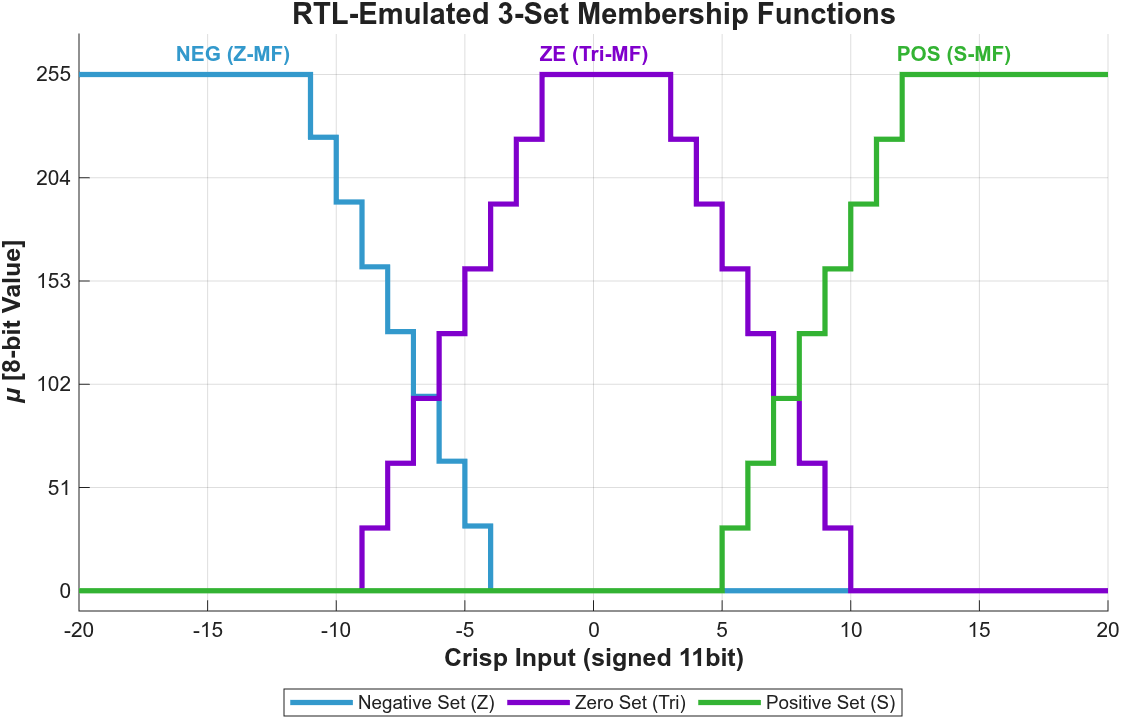
\includegraphics[width=\columnwidth]{./images/matlab/fuzzy_sets.png}
\caption{RTL-emulated 3-set membership functions, illustrating the Z-shaped, Triangular-shaped, and S-shaped structures.}
\label{fig:fuzzy_sets}
\end{figure}

\subsection{Defuzzification}
A Sugeno-type weighted average defuzzifies the inference
output into a crisp value, $\Delta D$:
\begin{equation}
    \Delta D = \frac{\sum_{i=1}^{n} w_i \cdot c_i}{\sum_{i=1}^{n} w_i}
    \label{eq:defuzzification}
\end{equation}
Here, $n$ is the active rule count, $w_i$ is 
the firing strength, and $c_i$ is the constant 
output coefficient. These $c_i$ values are 
hardware-encoded constants defined in tabular form 
corresponding to the five output 
fuzzy sets: \textbf{Big\_Decrease} (-16), 
\textbf{Decrease} (-4), 
\textbf{Hold} (0), \textbf{Increase} 
(4), and \textbf{Big\_Increase} (16). 

To eliminate the complex hardware division, 
a structure similar to Algorithm 
\ref{alg:mf_interpolation} is used. The 
denominator sum ($\sum w_i$) is mapped to its 
nearest power of 2, allowing the division to be 
replaced by an efficient bitwise right-shift. 
Furthermore, since the non-zero $c_i$ values are strictly 
powers of 2, the multiplication ($w_i \cdot c_i$) is precisely 
executed via simple bitwise shift operations, completely 
eliminating the need for hardware multipliers.

\section{Simulation and Results}
\label{sec:results}

The performance of the proposed fuzzy logic-based MPPT controller was validated through a comprehensive simulation conducted in MATLAB/Simulink. The total simulation time was 0.6 seconds, divided into three distinct sections to demonstrate the controller's performance during both steady-state and transient conditions. 

The PV efficiency, calculated as $P_{pv}/P_{pvmax}$, is the primary metric for evaluating the MPPT algorithm's effectiveness. The converter efficiency is evaluated as $P_{bat}/P_{pv}$. Due to the absence of signal filtering in the measurement blocks, instantaneous efficiency readings can momentarily appear above 100\% during sharp transients.

\textbf{Phase 1: Initial Stabilization (0s - 0.2s):} During the first 0.2 seconds, the system operates with a manual, fixed duty cycle setting. The fuzzy logic controller is not active, allowing the converter to stabilize. The overall simulation results across the full 0.6 seconds, illustrating this initial phase, are depicted in Figure \ref{fig:matlab_sim_overall}.

\begin{figure}[ht]
\centering

\includegraphics[width=\columnwidth]{./images/matlab/matlabsimresult.jpg}
\caption{Overall MATLAB simulation results across the three performance phases.}
\label{fig:matlab_sim_overall}
\end{figure}

\textbf{Phase 2: Fuzzy Controller Activation (0.2s):} At 0.2 seconds, the fuzzy logic MPPT controller is activated. Figure \ref{fig:sim_zoom_02} provides a zoomed-in view of this specific moment in time. The controller rapidly adjusts the duty cycle to bring the system to the maximum power point (MPP), achieving over 99\% PV efficiency in just 13.4 milliseconds.

\begin{figure}[ht]
\centering

\includegraphics[width=\columnwidth]{./images/matlab/matlab_sim_result_around0_2.jpg}
\caption{Zoomed-in view of the FLC activation at 0.2s, showing rapid convergence to MPP.}
\label{fig:sim_zoom_02}
\end{figure}

\textbf{Phase 3: Transient Response (0.4s):} At 0.4 seconds, the solar irradiance is dropped from 1000 $W/m^2$ to 500 $W/m^2$ to evaluate the effect of sudden environmental changes. Figure \ref{fig:sim_zoom_04} shows the zoomed-in transient response. Despite the disturbance causing a momentary dip in PV efficiency, the fuzzy controller responds swiftly, restoring the efficiency to over 99\% in approximately 1 millisecond.

\begin{figure}[ht]
\centering

\includegraphics[width=\columnwidth]{./images/matlab/matlab_sim_result_around0_4.jpg}
\caption{Zoomed-in view of the transient response at 0.4s during an irradiance drop from 1000 to 500 $W/m^2$.}
\label{fig:sim_zoom_04}
\end{figure}

These individual observations confirm the robustness and high performance of the fuzzy logic controller, showcasing its ability to quickly track the MPP and maintain high efficiency, even under rapidly changing environmental conditions.

Table \ref{tab:steady_state_results} summarizes the steady-state performance of the proposed system under the evaluated varying irradiance conditions. The results demonstrate that the fuzzy logic controller maintains exceptional PV tracking efficiency while the buck converter sustains high power conversion efficiency across varying environmental states. Notably, the PV efficiency and buck converter efficiency remain around 99\% and 95\%, respectively, up until the converter enters Discontinuous Conduction Mode (DCM) at very low irradiance levels, which explains the efficiency drop observed at 200 $W/m^2$.

\begin{table}[htbp]
    \centering
    \caption{Steady-State Performance Metrics}
    \label{tab:steady_state_results}
    \begin{tabular}{|l|c|c|c|}
        \hline
        \textbf{Irradiance ($W/m^2$)} & \textbf{1000} & \textbf{500} & \textbf{200} \\
        \hline
        \textbf{PV Efficiency (\%)} & 99.3 & 99.1 & 99.0 \\
        \hline
        \textbf{Buck Converter Efficiency (\%)} & 95.2 & 94.9 & 78.8 \\
        \hline
    \end{tabular}
\end{table}

\section{Conclusions}
\label{sec:conclusion}
This paper presents an ASIC-oriented, three-input fuzzy logic MPPT controller for PV battery chargers that evaluates changes in PV voltage, output current, and absolute PV voltage to achieve highly responsive tracking. A major contribution is the proposed hardware-efficient architecture that replaces complex multipliers and dividers with simple look-up tables and bitwise shifts, significantly reducing implementation complexity for low-cost IC design. Simulation results demonstrate over 99\% PV tracking efficiency and validate the effectiveness of this approach compared to previous 2-input systems (Table \ref{tab:comparison}). The three-input architecture eliminates local minima trapping and maintains high steady-state stability at 500 kHz switching frequency, providing a favorable trade-off between tracking accuracy, transient response, and hardware complexity.

\begin{table}[h]
\centering
\caption{Comparison Between Previous 2-Input FLC and Proposed 3-Input FLC}
\label{tab:comparison}
\begin{tabular}{|l|c|c|}
\hline
\textbf{Parameter} & \textbf{Previous Work} & \textbf{Proposed Work} \\ \hline
FLC Type & Mamdani & Sugeno \\ \hline
PV Tracking Efficiency & $\approx$ 97\% & $> 99\%$ \\ \hline
Buck Conv. Efficiency & $\approx$ 96\% & $\approx$ 95\% \\ \hline
Switching Frequency & 10 kHz & 500 kHz \\ \hline
Settling Time & $>50ms$ &  $<15ms$ \\ \hline
IC Area Optimization & Multiplier-based & LUT \& Bitwise Shifts \\ \hline
\end{tabular}
\end{table}

The proposed approach provides a favorable trade-off between tracking accuracy, transient response, and hardware complexity, highlighting its suitability for low-cost ASIC implementations. Future work will focus on the complete physical integrated circuit (IC) implementation and experimental hardware validation of the proposed system.
To promote reproducibility and encourage further research, the complete MATLAB/Simulink models and associated code developed for this study are publicly available at \url{https://github.com/mehmetgok1/MATLAB}.
\begin{thebibliography}{99}

\bibitem{DeSoto2006} W. De Soto, S.A. Klein, and W.A. Beckman, "Improvement and validation of a model for photovoltaic array performance," Solar Energy, vol. 80, no. 1, pp. 78--88, 2006.

\bibitem{EricksonBook} R. Erickson and D. Maksimovic, "Fundamentals of Power Electronics," 2nd ed. Springer, 2001.

\bibitem{RashidBook} M. H. Rashid, "Power Electronics Handbook," 4th ed. Butterworth-Heinemann, 2017.

\bibitem{TIReport} Texas Instruments, "Basic Calculation of a Buck Converter," Application Report SLVA477B, 2015.

\bibitem{mppt_book} Z. Dalala, Z. U. Zahid, H. Y. Kanaan, N. M. L. Ha, and D. C. Habineza, "Design and real-time implementation of a novel photovoltaic MPPT system," IEEE Trans. Sustain. Energy, vol. 7, no. 3, pp. 1101–1115, Jul. 2016.

\bibitem{fuzzy_review} T. S. Ubale and S. V. Chaudhari, "Review on fuzzy logic based MPPT for photovoltaic systems," in Proc. IEEE Int. Conf. Elect. Eng. Technol. (ICETECH), 2016, pp. 1–6.

\bibitem{zadeh} L. A. Zadeh, "Fuzzy sets," Inf. Control, vol. 8, no. 3, pp. 338–353, 1965.

\bibitem{po_ic} D. P. Hohm and M. E. Ropp, "Comparative study of maximum power point tracking algorithms," Prog. Photovolt. Res. Appl., vol. 11, no. 1, pp. 47–62, 2003.

\end{thebibliography}

\end{document}